
%\documentclass{report}
\documentclass{article}
%\documentclass{scrartcl}

%\usepackage{mslapa}
\usepackage{hyperref}
\usepackage{amsmath}
\usepackage{graphicx}
\usepackage{ulem}
\usepackage{vmargin}
\usepackage{tabularx}
\usepackage{sectsty}
\usepackage{pbox}
\usepackage{bigstrut}
\usepackage{enumerate}
\usepackage{listings}
\usepackage{parskip}   % space paragraphs but dont indent
\usepackage{verbatim}  % \verbatiminput{file}
\usepackage{gensymb}
\usepackage{color}

\usepackage{natbib}

%\setpapersize{USletter}
%\sectionfont{\normalsize}
%\subsectionfont{\normalsize}
\setmarginsrb{1.0in}{1.0in}{1.0in}{1.0in}{0in}{0.25in}{0in}{0.20in}

% configure \bigstrut size
% This configures spacing above and below rows in a tabularx.
\renewcommand{\bigstrutjot}{2.0\jot}

\providecommand{\e}[1]{\ensuremath{\times 10^{#1}}}

\raggedright

\begin{document}

% {{{ Title Page

\title{Lab 3 (EECE 344)}
\date{March 24, 2012}
\author{Jeremiah Mahler}

\maketitle
% }}}

\tableofcontents

\pagebreak

% {{{ Introduction
\section{Introduction}

The device described here shows how to construct a bus
using a Lattice MachXO\cite{EB66} board which connects
to leds, switches and multiple ram memory chips.
And how to control reads/writes to this bus
over SPI by an ARM STM32L Discovery\cite{UM1079} board.

% }}}

% {{{ Pin Assignments, Schematics
\section{Pin Assignments, Schematics}
\label{sec:pa}

The pin assignments define all the interconnecting wires
between the ARM, CPLD and other components.

% describe the pin meanings
To locate a pin on the CPLD requires two designations\citep[Pg. 11-14]{EB66}.
The first is the header which has names such as J9, J7, etc.
And the second is the number of the pin.
The board will have pin numbers at the begining and end of a header
to denote the orientation.

On the CPLD the pins correspond to headers (J9, J7, etc)
and pins within those headers\citep[Pg. 11-14]{EB66}.
The header and pin numbers are printed at the end of each header.

When specifiying the pin constraints in Diamond\cite{Diamond}
the header and pin number are not available.
Instead the "Mach XO Ball" must be specified.
And this value is included in the following pin assignments.

The pin assignments are given in Tables
\ref{tbl:ramcommon}, \ref{tbl:rampinsuniq}, \ref{tbl:pins}
as well as the schematic in Figure \ref{fig:ram_to_cpld}.

% {{{ RAM common Table
\begin{table}
\center
\begin{tabular}{|l|l|l|l|l|l|l|}
	\hline
	\multicolumn{3}{|c|}{\textbf{RAM}} & \multicolumn{4}{|c|}{\textbf{CPLD}} \\
	\hline
	pin & label & description &  function & Mach XO Ball & Header & Pin \\
	\hline
	12 & A0 & mem\_address & PL17D & L4 & J4 & 36 \\
	\hline
	11 & A1 & mem\_address & PL12D & L2 & J4 & 35 \\
	\hline
	10 & A2 & mem\_address & PL17C & L5 & J4 & 34 \\
	\hline
	9 & A3 & mem\_address & PL12C & K2 & J4 & 33 \\
	\hline
	8 & A4 & mem\_address & PL15C & M2 & J4 & 26 \\
	\hline
	7 & A5 & mem\_address & PL10C & G1 & J4 & 21 \\
	\hline
	6 & A6 & mem\_address & PL10D & H1 & J4 & 23 \\
	\hline
	5 & A7 & mem\_address & PL8D & H3 & J4 & 19 \\
	\hline
	27 & A8 & mem\_address & PL15D & N2 & J4 & 28 \\
	\hline
	26 & A9 & mem\_address & PL11C & J3 & J4 & 29 \\
	\hline
	23 & A10 & mem\_address & PL19A & N4 & J4 & 38 \\
	\hline
	25 & A11 & mem\_address & PL11D & K3 & J4 & 31 \\
	\hline
	4 & A12 & mem\_address & PL8C & G3 & J4 & 17 \\
	\hline
	28 & A13 & mem\_address & PL16D & R2 & J4 & 32 \\
	\hline
	3 & A14 & mem\_address & PL7C & E1 & J4 & 13 \\
	\hline
	31 & A15 & mem\_address & PL7D & F1 & J4 & 15 \\
	\hline
	2 & A16 & mem\_address & PL6D & D1 & J4 & 11 \\
	\hline
	13 & DQ0 & mem\_data & PL7A\_LV\_T & F2 & J3 & 25 \\
	\hline
	14 & DQ1 & mem\_data & PL17A\_LV\_T & K5 & J3 & 32 \\
	\hline
	15 & DQ2 & mem\_data & PL18A\_LV\_T & M5 & J3 & 38 \\
	\hline
	17 & DQ3 & mem\_data & PL9A\_LV\_T & H4 & J3 & 37 \\
	\hline
	18 & DQ4 & mem\_data & PL8A\_LV\_T & G4 & J3 & 31 \\
	\hline
	19 & DQ5 & mem\_data & PL16A\_LV\_T & J4 & J3 & 26 \\
	\hline
	20 & DQ6 & mem\_data & PL15A\_LV\_T & L3 & J3 & 20 \\
	\hline
	21 & DQ7 & mem\_data & PL5A\_LV\_T & B1 & J3 & 19 \\
	\hline
	32 & Vcc & suppy voltage & & & J9 & 5 \\
	\hline
	16 & Vss & ground & & & J3 & 36 \\
	\hline
\end{tabular}
\caption{Pin assignments between RAM chip and the CPLD
which are common to both chips.
See Table \ref{tbl:rampinsuniq} for those pins which are
unique for each chip.
}
\label{tbl:ramcommon}
\end{table}
% }}}

% {{{ RAM unique Table
\begin{table}
\center

\begin{tabular}{|l|l|l|l|l|l|l|l|}
    \hline
	\multicolumn{4}{|c|}{\textbf{RAM \#1}} & \multicolumn{4}{|c|}{\textbf{CPLD}} \\
	\hline
    pin & label & variable & description &  function & Mach XO Ball & Header & Pin \\
    \hline
    30 & CE2 & mem1\_ce2 & chip enable & PL14C & N1 & J4 & 37 \\
	\hline
    22 & CE\# & mem1\_ceh\_n & chip enable & PL19B & N3 & J4 & 40 \\
	\hline
    29 & WE\# & mem1\_we\_n & write enable & PL14D & P1 & J4 & 39 \\
	\hline
    24 & OE\# & mem1\_oe\_n & output enable & PL16C & R1 & J4 & 30 \\
	\hline
\end{tabular}

\vspace{5mm}  

\begin{tabular}{|l|l|l|l|l|l|l|l|}
    \hline
	\multicolumn{4}{|c|}{\textbf{RAM \#2}} & \multicolumn{4}{|c|}{\textbf{CPLD}} \\
	\hline
    pin & label & variable & description &  function & Mach XO Ball & Header & Pin \\
    \hline
    30 & CE2 & mem2\_ce2 & chip enable & PL8B & G5 & J3 & 33 \\
	\hline
    22 & CE\# & mem2\_ceh\_n & chip enable & PL11B & J2 & J3 & 4 \\
	\hline
    29 & WE\# & mem2\_we\_n & write enable & PL19B & H5 & J3 & 39 \\
	\hline
    24 & OE\# & mem2\_oe\_n & output enable & PL18B & M4 & J3 & 40 \\
	\hline
\end{tabular}

\caption{Pin assignments between RAM chip and the CPLD
which are unique to each RAM chip.}
\label{tbl:rampinsuniq}
\end{table}
% }}}

\begin{figure}
\center
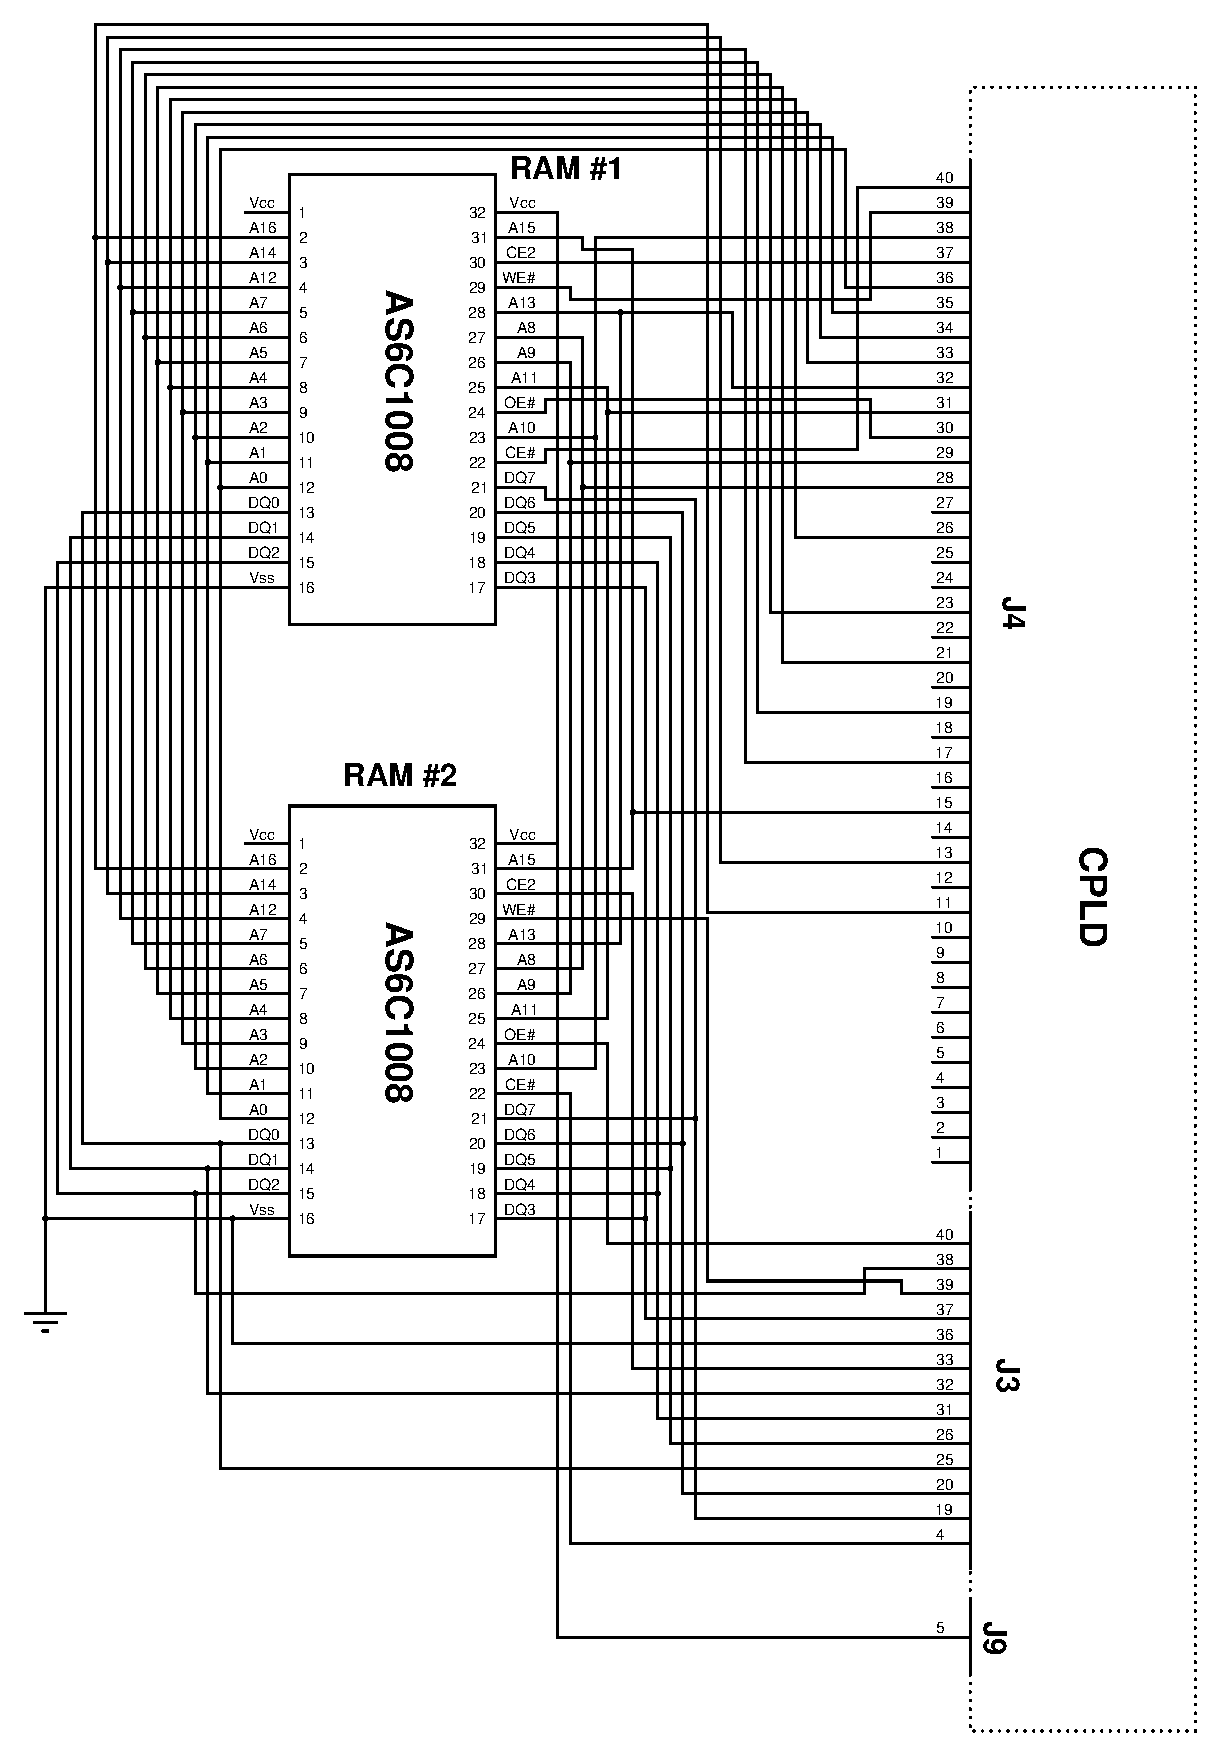
\includegraphics[scale=0.7]{figures/schematics/RAM_to_CPLD}
\caption{Schematic diagram of wires between both RAM chips and
the CPLD.}
\label{fig:ram_to_cpld}
\end{figure}

\begin{figure}
\center
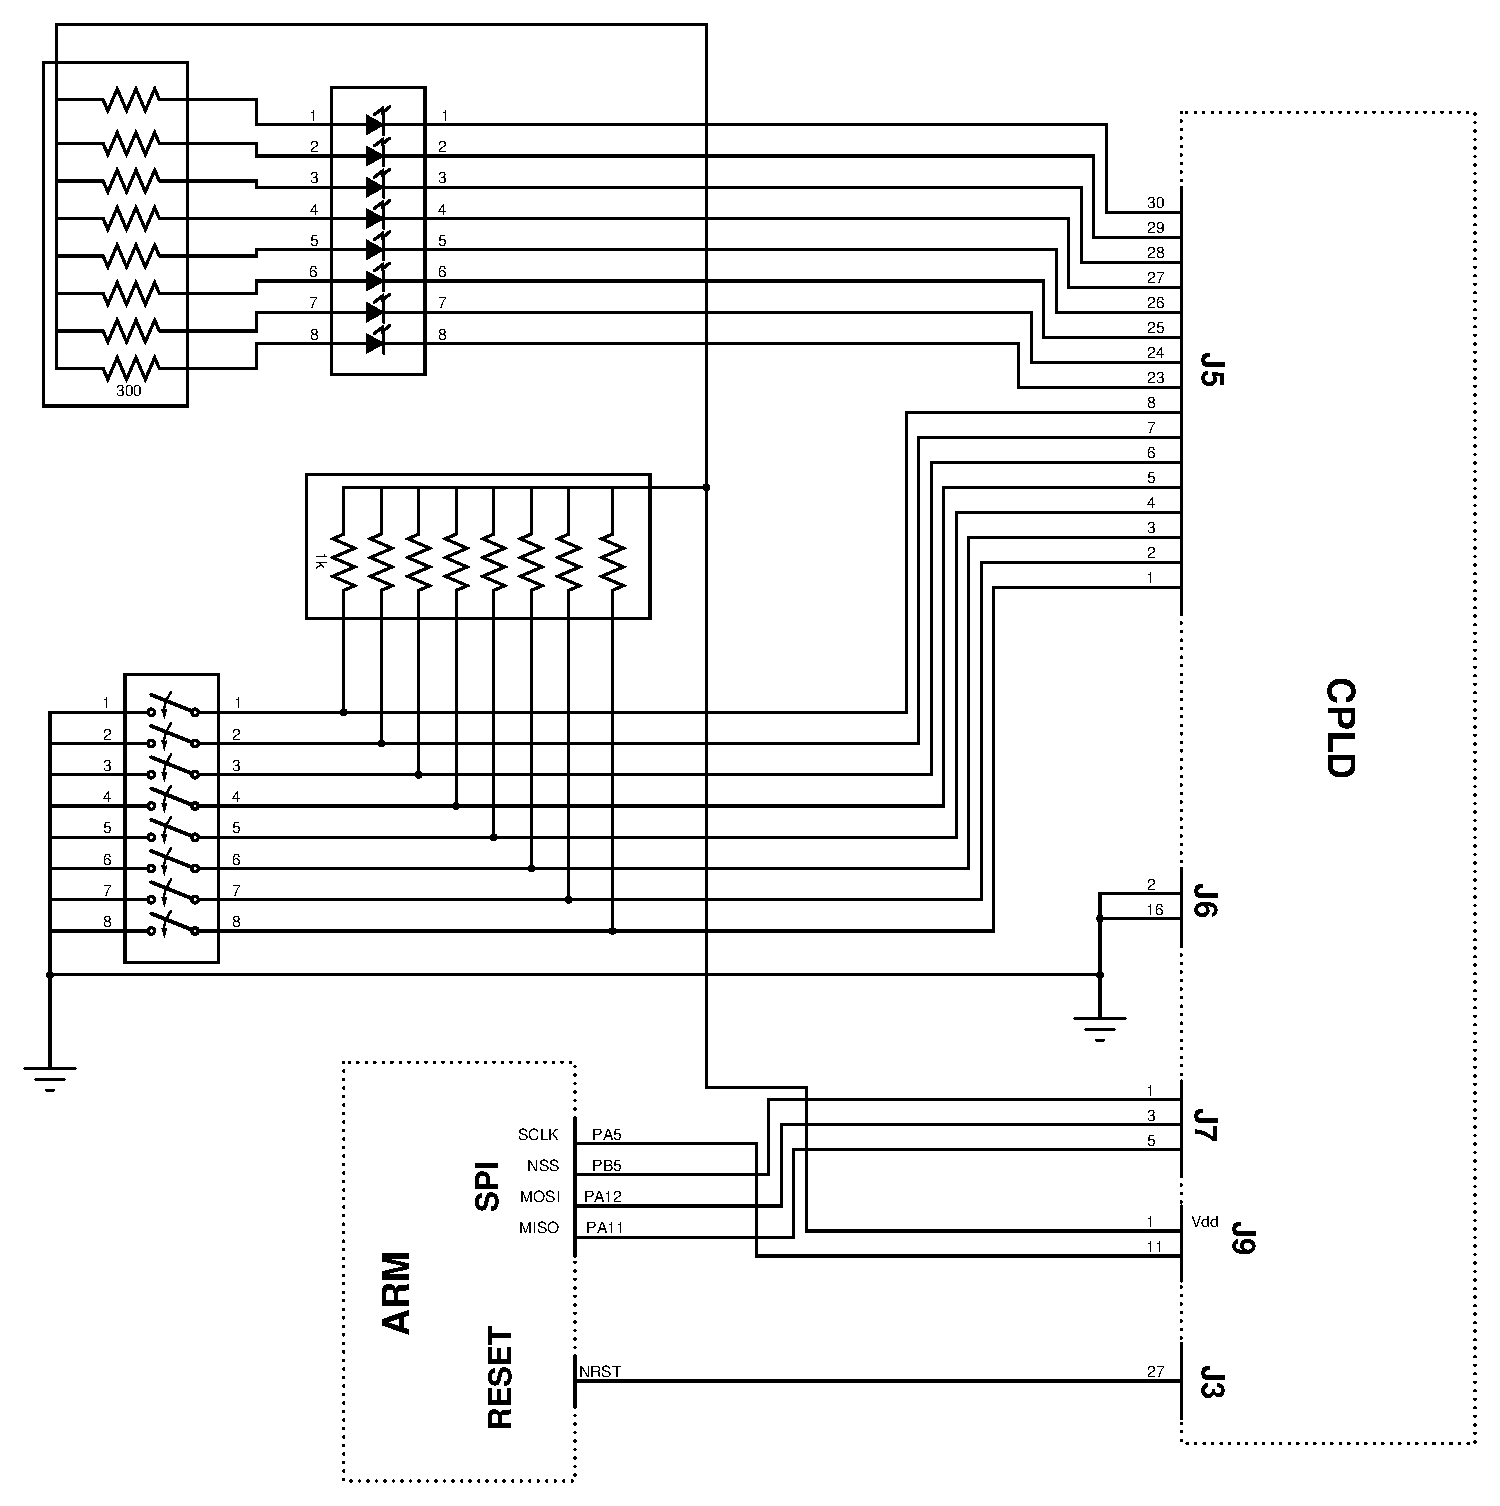
\includegraphics[scale=0.7]{figures/schematics/SPI_LEDs_SW}
\caption{Schematic diagram of wires between the ARM and the CPLD.}
\label{fig:arm_to_cpld}
\end{figure}

\begin{table}
\center
\begin{tabular}{|l|l|l|}
    \hline
    \multicolumn{3}{|c|}{\textbf{Memory Map}} \\
    \hline
    address (hex) & name & variable \\
    \hline
    0x74 & switches & switch\_ce\_n \\
    0x6C & bar leds & bar\_led\_ce\_n \\
    0x50 - 0x5F & RAM \#2 & mem2\_ce\_n \\
    0x2F & board leds & board\_led\_ce\_n \\
    0x00 - 0x0F & RAM \#1 & mem1\_ce\_n \\
    \hline
\end{tabular}
\caption{Device memory map.}
\label{tbl:memmap}
\end{table}

% {{{ pins Table
\begin{table}
	\center
	\begin{tabular}{|l|l|l|l|l|l|l|}
		\hline
		\multicolumn{7}{|c|}{\textbf{SPI}} \\
		\hline
		\multicolumn{1}{| c |}{\textbf{Verilog}} &
		\multicolumn{1}{| c |}{} &
		\multicolumn{1}{| c |}{\textbf{ARM}} &
		\multicolumn{4}{| c |}{\textbf{CPLD}} \\
		\hline
		name & description & pin  &  function & Mach XO Ball & Header & Pin \\
		\hline
		SCLK & SPI clock & PA5 & PT9B & D7 & J9 & 11 \\
		NSS & SPI slave select & PB5 & PR4C & F13 & J7 & 1 \\
		MOSI & SPI master out slave in & PA12 & PR4D & F12 & J7 & 3 \\
		MISO & SPI master in slave out & PA11 & PR5C  & B16 & J7 & 5 \\
		\hline
		\multicolumn{7}{|c|}{\textbf{switches}} \\
		\hline
		\multicolumn{1}{| c |}{\textbf{Verilog}} &
		\multicolumn{1}{| c |}{} &
		\multicolumn{1}{| c |}{\textbf{input switches}} &
		\multicolumn{4}{| c |}{\textbf{CPLD}} \\
		\hline
		name & description & pin  &  function & Mach XO Ball & Header & Pin \\
		\hline
		switches[0] & input switch 8 & 8 & PT2C & B2 & J5 & 1 \\
		switches[1] & input switch 7 & 7 & PT9A & D8 & J5 & 2 \\
		switches[2] & input switch 6 & 6 & PT2D & B3 & J5 & 3 \\
		switches[3] & input switch 5 & 5 & PT9C & E8 & J5 & 4 \\
		switches[4] & input switch 4 & 4 & PT3A & A2 & J5 & 5 \\
		switches[5] & input switch 3 & 3 & PT9D & E9 & J5 & 6 \\
		switches[6] & input switch 2 & 2 & PT3B & A3 & J5 & 7 \\
		switches[7] & input switch 1 & 1 & PT10A & A10 & J5 & 8 \\
		          & power, Vdd, pull up &      &     &    & J9 & 1 \\
		          & ground &  & & & J6 & 2 \\
		\hline
		\multicolumn{7}{|c|}{\textbf{LEDs}} \\
		\hline
		\multicolumn{1}{|c|}{\textbf{Verilog}} &
		\multicolumn{1}{|c|}{} &
		\multicolumn{1}{|c|}{\textbf{output LEDs}} &
		\multicolumn{4}{|c|}{\textbf{CPLD}} \\
		\hline
		name & description & pin  &  function & Mach XO Ball & Header & Pin \\
		\hline
%		bar\_leds[10] & output led 10 & 10 & PT5C & B4 & J5 & 21 \\
%		bar\_leds[9] & output led 9 & 9 & PT12A & A11  & J5 & 22 \\
		bar\_leds[0] & output led 8 & 8 & PT15D & B5   & J5 & 23 \\
		bar\_leds[1] & output led 7 & 7 & PT12B & A12  & J5 & 24 \\
		bar\_leds[2] & output led 6 & 6 & PT6E  & E7   & J5 & 25 \\
		bar\_leds[3] & output led 5 & 5 & PT12C & B11  & J5 & 26 \\
		bar\_leds[4] & output led 4 & 4 & PT6F  & E6   & J5 & 27 \\
		bar\_leds[5] & output led 3 & 3 & PT12D & B12  & J5 & 28 \\
		bar\_leds[6] & output led 2 & 2 & PT16C & A5   & J5 & 29 \\
		bar\_leds[7] & output led 1 & 1 & PT13C & C11  & J5 & 30 \\
		          & power, Vdd, pull up &      &     &    & J9 & 1 \\
		          & ground &  & & & J6 & 16 \\
		\hline
		\multicolumn{7}{|c|}{\textbf{reset}} \\
		\hline
		\multicolumn{1}{| c |}{\textbf{Verilog}} &
		\multicolumn{1}{| c |}{} &
		\multicolumn{1}{| c |}{\textbf{ARM}} &
		\multicolumn{4}{| c |}{\textbf{CPLD}} \\
		\hline
		name & description & pin  &  function & Mach XO Ball & Header & Pin \\
		\hline
		reset\_n & active low reset & NRST & PL7B & G2 & J3 & 27 \\
		\hline
	\end{tabular}
	\caption{Definition of the pin assignments between the ARM board,
		the CPLD, and other devices.
        Notice that the switch and LEDs are reversed.
        This was done so that the orientation from LSB to MSB is from
        right to left.
        }
	\label{tbl:pins}
\end{table}
% }}}

% configuring using Diamond
The pins were configured with standard options:
low voltage 3.3 volt CMOS with no pull up or pull down.
Output pins to drive the leds were configured for 8 mA drive current.

% input switches
The input switches to the CPLD can be interfaced by connecting
one end to ground and the other end to the pin along with a
pull up resistor to Vdd.
A resistor value between 1k and 10k should be acceptable.
And the pull up voltage for Vdd can be sourced from a pin on
the board (Table \ref{tbl:pins}).

% output leds
The output LEDs are connected to the CPLD using a series
resistor.
Vdd would connect to the resistor which connects to the led
(forward biased) which connects to the pin.
The value of the resistor should limit the current to approximately
10 mA.
A value of 300 $\ohm$ is a typical value.

% reset pin
To reset the boards their reset pins must be configured.
The ARM board provides a \verb+NRST+ pin which is at Vcc
when enabled and goes low when the reset button is pushed\cite[Pg. 17, 20]{UM1079}.
This can then be connected to the CPLD to cause
it to reset using \verb+GSRN+\citetext{\citealp[Pg. 13, 46, 50, 53]{DS1002}; \citealp[Pg. 8]{EB66}}.
Table \ref{tbl:pins} lists the exact pins that were used.

\clearpage

% }}}

% {{{ SPI protocol
\section{SPI protocol}

Communication with the "bus" on the CPLD is accomplished using SPI
\citetext{ \citealp[Pg. 278]{cady2009microcontrollers}; \citealp[Pg. 665]{STRM0038}}.
For the bus there are two required operations: read and write.
And in order to perform these operations it requires a minimum of
two transactions over the SPI.
A read, for example, would send the address in the first transaction.
And in the second transaction the data read would be returned.
A write is similar except that for the second transaction the
data to be written is sent.
The format of the transaction is defined in Table \ref{tbl:spiformat}.

\begin{table}
\center
\begin{tabular}{|c|c|c|}
    \multicolumn{1}{l}{8} & \multicolumn{1}{l}{7} & \multicolumn{1}{r}{1} \\
\hline
rw bit & \multicolumn{2}{|c|}{address} \\
\hline
\multicolumn{3}{|c|}{data} \\
\hline
\end{tabular}
\caption{Format of two byte SPI transactions.}
\label{tbl:spiformat}
\end{table}

This implementation has the SPI settings hard coded as shown
in Table \ref{tbl:spi}.
Both the ARM and the CPLD must use these same settings in order
to work properly with each other.

\begin{table}
\center
\begin{tabular}{|l|l|}
	\hline
	option & value \\
	\hline
	MSB & first \\
	CPOL & 0 \\
	CPHA & 0 \\
	NSS & slave select\\
	\hline
\end{tabular}
\caption{SPI configuration options}
\label{tbl:spi}
\end{table}

A complication of this two byte protocol pertains to how to
determine which byte is the first and which is the second.
The method used here is to modify the SPI protocol so that the NSS
signal is held active across two bytes instead of just one.
This solution requires no additional hardware and is straight forward
to implement in the CPLD.

Because the SPI is full duplex process a byte is sent and received
on every transaction.
Because of this some values are ignored in certain situations.
For example, during a read operation, the address is sent
first, then a second byte must be sent in order to get
the received value.
The second value sent is ignored and could be any value.

For a detailed timing diagram of the read and write operations refer
to Figures \ref{fig:spi_read} and \ref{fig:spi_write}.

\begin{figure}
\center
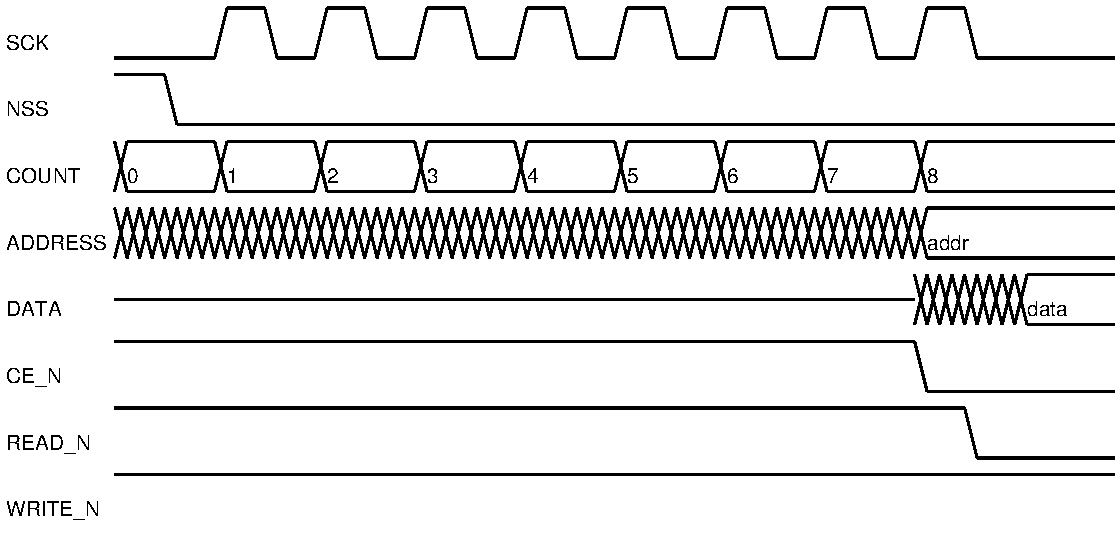
\includegraphics[scale=0.7]{figures/spi_ctl-timing/read-byte1} \\
(a) \\
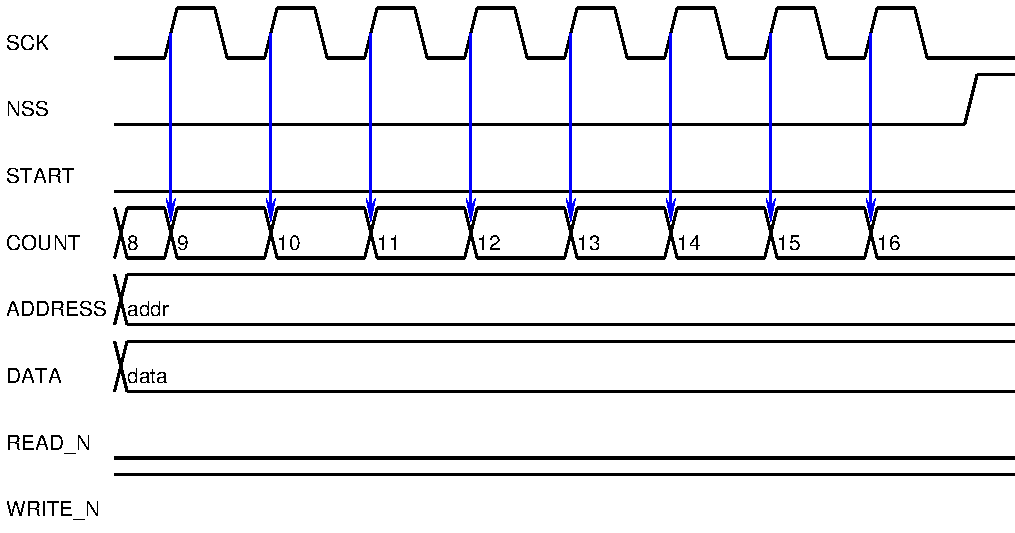
\includegraphics[scale=0.7]{figures/spi_ctl-timing/read-byte2} \\
(b)
\caption{Timing diagram of SPI read cycle.
Part (a) is the first 8-bits and part (b) is the second
8-bits continuing from (a).
Notice in part (a) where the ADDRESS is valid and READ\_N becomes active (low).
The data is not immediately read but instead it is delayed until
the negative edge of the SCK.
This is necessary for device such as RAM chips which may
require a short period of time to produce valid data.}
\label{fig:spi_read}
\end{figure}

\begin{figure}
\center
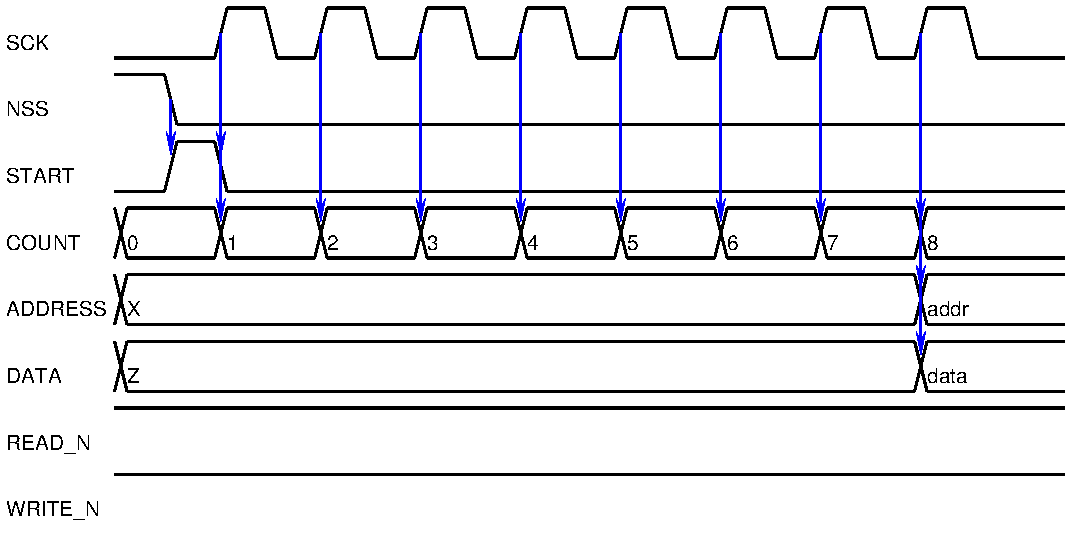
\includegraphics[scale=0.7]{figures/spi_ctl-timing/write-byte1} \\
(a) \\
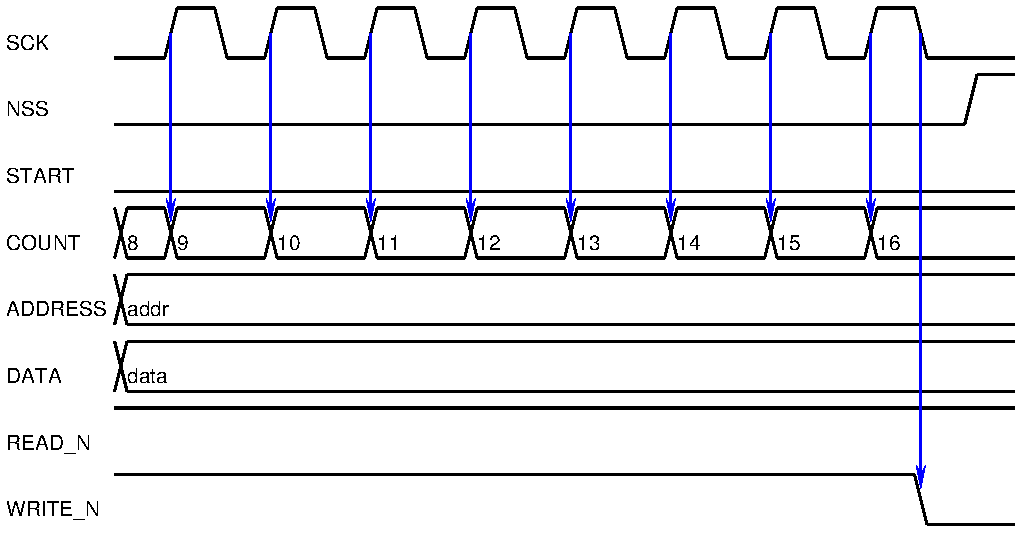
\includegraphics[scale=0.7]{figures/spi_ctl-timing/write-byte2} \\
(b)
\caption{Timing diagram of SPI write cycle.
Part (a) is the first 8-bits and part (b) is the second
continuing from (a).
A write is not initiated until the end of the
second byte because it has to read this byte entirely before it can be written.}
\label{fig:spi_write}
\end{figure}

When values are read or written to the bus they must be held for
some amount of time.
In this implementation this is accomplished by controlling the
pulse width from the end of the 16'th \verb+sck+ edge and the positive
edge of \verb+nss+ (going disabled).
Since the clock speed of the SPI is on the order of kHz and the
clock inside the CPLD is on the order of MHz there should be plenty
of time for any memory timings or other operations to be done.

\clearpage

% }}}

% {{{ User Interface
\section{User Interface}

In order for the user to be able to perform read and write
operations to the bus devices an interface needs to be defined.
The only means of input is using an eight position DIP switch.
Outputs are provided by an LCD, a bar of eight LEDS,
and a group of eight LEDs on board the CPLD.

The bar of LEDs and the group of LEDs on the CPLD both operate
similarly.
They act as an eight bit register which can be read from and written to.
Refer to Table \ref{tbl:memmap} for their specific addresses.

The LCD is the primary means of user feedback.
It instructs the user when to enter a command or data and
it displays the results.
Figure \ref{fig:armstate} gives an overview of the states of
the system.

\begin{figure}
\center
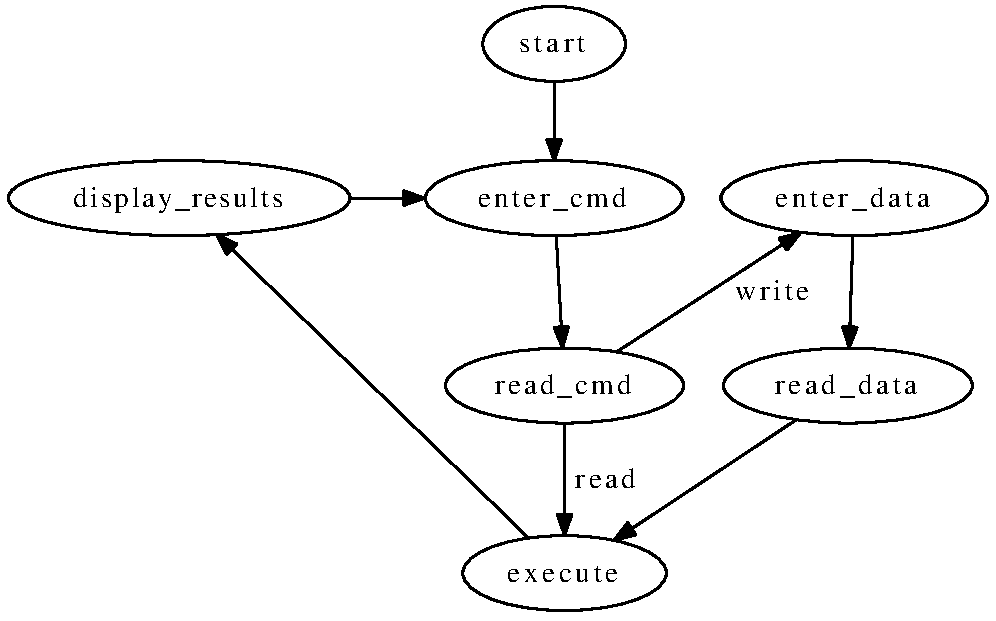
\includegraphics[scale=0.8]{figures/arm-state_diagram/arm-state_diagram}
\caption{State diagram of ARM board operation.
The states 'display\_results', 'enter\_cmd' and 'enter\_data'
wait for the user set the input switches as necessary and then press
the user button.
'read\_cmd' reads the input switches to get the command (address and rw bit).
If the command is a write 'read\_data' reads the switches again to get the data.
And 'execute' performs the read/write command.
}
\label{fig:armstate}
\end{figure}

As an example of reading the switches.
Notice that the only difference is the inclusion of the
rw bit as part of the data value whereas the address
is only 7-bits and excludes this part.
\begin{verbatim}
CMD
74 R F4
\end{verbatim}

Refer to the memory map (Table \ref{tbl:memmap}) for
a complete list of the addresses that can be read from and written
to.

% }}}

% {{{ Conclusion
\section{Conclusion}
% difficulties

% }}}

% {{{ References
\clearpage

\pagebreak
\renewcommand*{\refname}{\vspace{-8mm}}
\section{References}
%\bibliographystyle{ieeetr}
\bibliographystyle{plain}
\bibliography{references}
% }}}

\end{document}

% vim:foldmethod=marker

